\documentclass[a4paper,12pt]{report}

\usepackage[french]{babel}
\usepackage[french]{varioref}
\usepackage[T1]{fontenc}
\usepackage[utf8]{inputenc}
\usepackage{mathtools}
\usepackage{graphicx}
\usepackage{amssymb,bm}
\usepackage{tikz,tkz-tab}
\usepackage{mathtools,bm}
\usepackage{url}
\usepackage{lmodern}
\usepackage{textcomp}
\usepackage{amsmath}
\newenvironment{spmatrix}[1]
 {\def\mysubscript{#1}\mathop\bgroup\begin{pmatrix}}
 {\end{pmatrix}\egroup_{\textstyle\mathstrut\mysubscript}}
 \renewcommand{\thesection}{\arabic{section}}
\usepackage{hyperref}
\usepackage{pdfpages}
\usepackage[top=2cm,bottom=2cm,left=2cm,right=2cm]{geometry}
\title{}
\date{}
\begin{document}

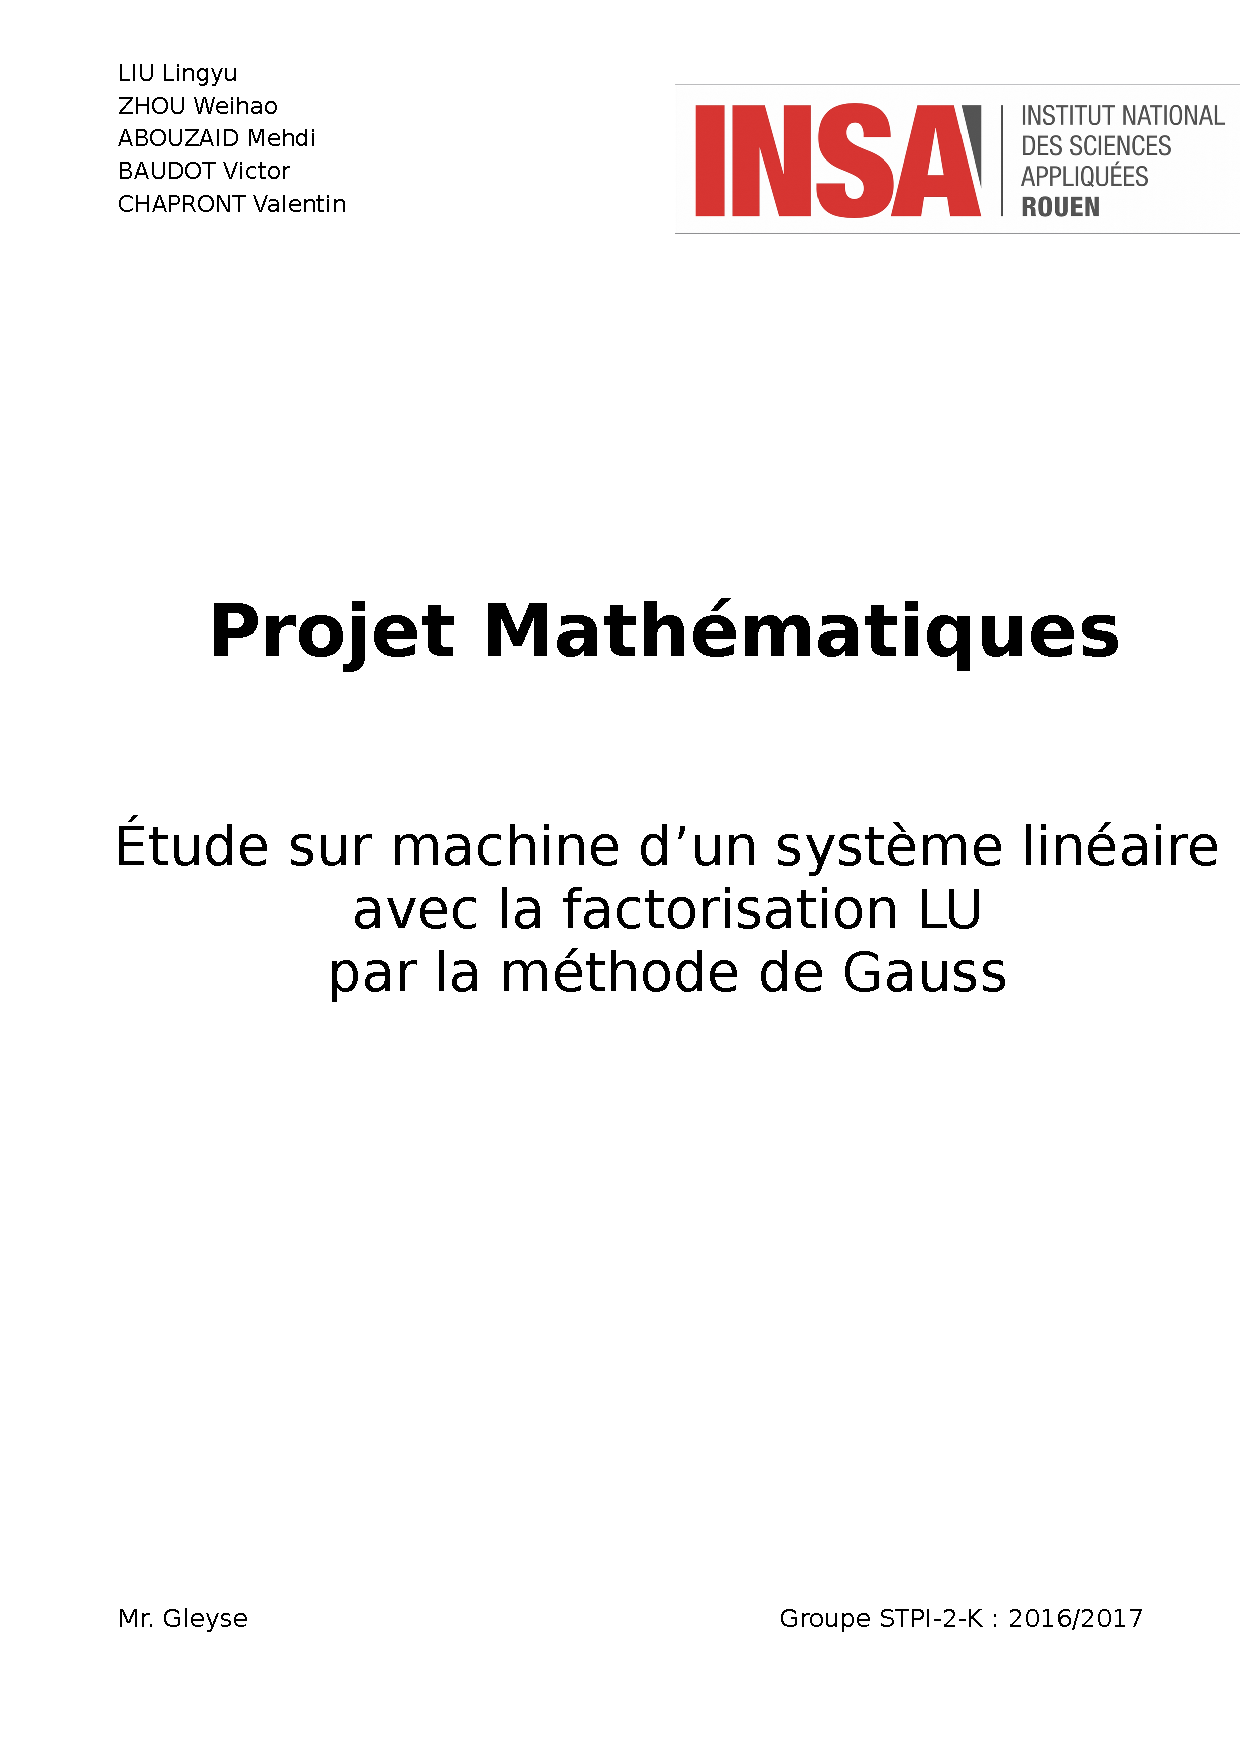
\includepdf{presentation.pdf}
\tableofcontents

\newpage

\chapter*{Introduction}


Depuis le collège, nous nous intéressons à la résolution de systèmes linéaires. Tout d'abord assez simples, celles-ci sont rapidement devenus de plus en plus compliquées et aujourd’hui nous nous appliquons à résoudre des systèmes linaires grâce à la factorisation LU et à la méthode de Gauss.\\

Ces méthodes de résolution des systèmes linaires ont progressivement été mis au point au cours de l'Histoire. Mais ce n'est que très récemment(sur l'échelle de l'Humanité), que la méthode de Gauss utilisant la factorisation LU a vu le jour. Nous expliquerons plus en détail les origines de sa création dans la première partie. Nous partirons des débuts de l'algorithmie pour voir son évolution jusqu'à la mise en place de la méthode de Gauss-Jordan.\\

La méthode de Gauss vise en fait à triangulariser une matrice en décomposant la matrice sous la forme LU avec L une matrice triangulaire inférieure à diagonale unité et U une matrice triangulaire supérieure. Nous développerons son fonctionnement dans la partie suivante en nous attardant sur le pivot de Gauss et l'inverse d'une matrice par la méthode de Gauss.\\

Grâce au programme que nous avons créé au cours du projet, nous avons pu mettre en application la méthode de Gauss et la factorisation LU pour résoudre différents systèmes linaires dont la matrice de Wilson et la matrice de Hilbert. La troisième partie de notre rapport sera donc consacré à présenter des exemples d'utilisation de la factorisation LU en utilisant notre programme écrit en Pascal. Nous y expliquerons également les programmes étudiés en cours.\\
\newpage

\chapter{L’algèbre linéaire de l’antiquité à nos jours}

Depuis des centaines d’années, des peuples s’intéressent aux mathématiques et à la résolution d’équations afin de résoudre certains problèmes liés à la vie quotidienne.\\

\section{La naissance de l'algèbre linéaire}
D’un côté, les Chinois se sont mis à résoudre des systèmes linéaires de 1er degré tandis que les Babyloniens et les Égyptiens résolvaient des problèmes pratiques du premier voire même du second degré. Les Grecs, quand à eux, n’ont pas fait évoluer les techniques de calcul car ils liaient leurs calculs à des constructions géométriques dont les solutions sont des fractions positives. D’autres peuples s’adonnaient aux mathématiques mais ce n’est que plusieurs siècles plus tard qu’on observe une forte avancée dans ce domaine, principalement dans la civilisation arabo-musulmane.\\ 

En effet, au IXème siècle, le célèbre savant Al-Khawarizmi énonce six équations canoniques dont il sait trouver la solution en utilisant les trois méthodes suivantes : le reboutement, la réduction ainsi que la division. Suite à la traductions des livres arabes dont celui d’Al-Khawarizmi, les recherches en mathématiques se propagent en Europe aux XV et XVIèmes siècle.\\ 

Un pont entre les deux branches des mathématiques: l’algèbre et la géométrie est alors réalisé par René Descartes lorsqu’il étudie des problèmes géométriques comme la détermination de l’intersection de deux droites en termes d’équations linaires. Après cette découverte majeure, les progrès en algèbre linéaire vont se limiter à des études ponctuelles comme la définition et l'analyse des premières propriétés des déterminants par Jean d'Alembert.\\

C’est à la fin du XVIIe siècle que, pour la première fois, se présentent des systèmes linéaires, avec des coefficients littéraux. Puis vers 1730, Maclaurin calcule explicitement les solutions de tels systèmes à 2 et 3 équations et donne également les formules pour 4 équations. Enfin, en 1750 Cramer écrit les formules générales pour un nombre quelconque d’équations sans toutefois en fournir de démonstration. Les formules de Cramer sont très efficaces mais les travaux d’Astronomie et de Géodésie conduisaient à des systèmes avec un nombre d’équations très important. Par exemple, pour 10 équations, la quantité d’opérations à effectuer est de l’ordre de 300 millions de multiplications. D’autres méthodes ont ainsi dû être mis en place comme la méthode du pivot de Gauss qui diminue le nombre d’opérations.\\

\section{La naissance du pivot de Gauss}
Gauss était très intéressé par l’astronomie et fut même nommé, en 1807, à l’âge de trente ans, directeur de l’Observatoire de Göttingen, poste qu’il gardera jusqu’à sa mort en 1855. \\

Lorsque l’astéroïde Pallas a été découvert par Olbers en 1809, Gauss s’y intéresse et se penche sur la détermination précise de son orbite. Il expliquera alors comment mettre en œuvre sa méthode des moindres carrés dans un mémoire qu’il publiera en 1810.\\
« A partir de six observations effectuées alors que la planète est en opposition- donc proche de la Terre -, Gauss obtient 12 équations entre 6 inconnues (l’anomalie moyenne, le mouvement diurne moyen, la longitude du nœud, l’inclinaison). Après l’obtention d’une solution approchée, il détermine 12 équations linéaires que doivent vérifier les rectifications à apporter aux 6 inconnues.  Rejetant en fait la dixième car trop imprécise compte que de l’observation, il dispose de 11 équations dont il tire 6 équations normales et finalement 6 corrections. »\\

Dans ce mémoire, Gauss formule certaines remarques pour faciliter la résolution algébrique du système linéaire formé par les équations normales. Ces remarques ne sont pas anodines car elles évoquent aujourd’hui pour nous la méthode d’élimination ou pivot de Gauss ainsi que la décomposition d’un polynôme de degré deux en somme de carrés.
Cette méthode, aussi nommée méthode d’élimination de Gauss-Jordan est une méthode dite directe car elle permet d’obtenir une solution à partir d’un nombre fini d’équations. Il s’agit d’obtenir un système (pas une matrice) avec le même nombre d’équations que d’inconnues.\\

Depuis Gauss, d’autres méthodes de résolution de systèmes linéaires, dites itératives (c’est-à-dire que ces méthode déterminent des solutions qui se rapprochent au fil des itérations de la solution recherchée) sont apparues comme celles de Jacobi en 1845 et de Cholesky en 1923. Cependant, nous traiterons dans ce rapport de la méthode du pivot de Gauss mais il est bon de noté que ces méthodes « itératives » permettent de limiter la propagation des erreurs par le biais des solutions successives lorsque le problème est mal conditionné ou contient un trop grand nombre de variables.\\

\newpage

\chapter{Analyse mathématique}
\section{Présentation du problème}

La résolution d’un système d’équations ainsi que l’inversion de matrices interviennent dans la plupart des problèmes mathématiques actuels, aussi bien dans la résolution de systèmes linéaires traditionnels que pour les résolutions numériques d’équations différentielles, de dérivées partielles,d’analyse de données etc.\\

Dans cette partie nous allons étudier l’inverse d’une matrice par la méthode de Gauss et la factorisation LU. Ces deux méthodes se rejoignent puisque d'un côté, la méthode de Gauss permet de trouver les solutions d’un système d’équations linéaires et de l'autre, la factorisation LU permet de triangulariser une matrice en la décomposant en deux matrices : une inférieure L et une supérieure U; ce n'est rien d'autre que la représentation matricielle de la méthode de Gauss.
\\

On cherche à résoudre le système suivant : 
\[
\left\{
\begin{array}{r  c l}
a_{11}x_1+a_{12}x_2+\cdots+a_{1n}x_n &=& b_1\\
a_{21}x_1+a_{22}x_2+\cdots+a_{2n}x_n &=& b_2\\
&\vdots&\\
a_{n1}x_1+a_{n2}x_2+\cdots+a_{nn}x_n &=& b_n
\end{array}
\right.
\]\\
Ce système de $n$ équations à $n$ inconnues est linéaires si les coefficients $a_{ij}$ sont constants et indépendants des inconnues $x_{j}$. \\

On peut aussi écrire ce système sous la forme :
$$\textbf{A x = b}$$
où \textbf{A} est la matrice du système, \textbf{x} le vecteur inconnu et \textbf{b} le vecteur second membre connu :
$$
\textbf{A}=\begin{pmatrix}
a_{11} & a_{12} & \cdots & a_{1n} \\
a_{21} & a_{22} & \cdots & a_{2n} \\
\vdots \\
a_{n1} & a_{n2} & \cdots & a_{nn} \\
\end{pmatrix}
\textbf{x}=\begin{pmatrix}
x_{1}\\
x_{2}\\
\vdots\\
x_{n}\\
\end{pmatrix}
\textbf{b}=\begin{pmatrix}
b_{1}\\
b_{2}\\
\vdots\\
b_{n}\\
\end{pmatrix}
$$\\
Les éléments de la matrice A sont désignés par $a_{i,j}$. Dans cette notation, $i$ désigne le numéro de la ligne et $j$ le numéro de la colonne. Ainsi $a_{i,j}$ est à l’intersection de la ligne $i$ et de la colonne $j$.
Quant aux vecteur $x$ et $b$, ils sont représentés par des matrices colonne regroupant leurs composantes. \\

Il existe trois grandes catégories de méthodes de résolution de systèmes d’équations :\\
- les méthodes du pivot (« directes ») pour les systèmes denses d’ordre peu élevé\\
- les décompositions de matrices en produit de type $A=LU$\\
- les méthodes itératives, adaptées aux systèmes non linéaires\\
\newpage
\section{Étude de la méthode mathématique du pivot de Gauss}

Les systèmes linéaires sont relativement simples d'un point de vue mathématiques, précisément en raison de la linéarité des équations. La méthode de Gauss est la méthode de résolution la plus simple et la plus commune; elle correspond à ce que l'on fait "à la main".\\

Pour décrire cette méthode, on reprends le système précédent : 
\[
\left\{
\begin{array}{r  c l}
a_{11}x_1+a_{12}x_2+\cdots+a_{1n}x_n &=& b_1\\
a_{21}x_1+a_{22}x_2+\cdots+a_{2n}x_n &=& b_2\\
&\vdots&\\
a_{n1}x_1+a_{n2}x_2+\cdots+a_{nn}x_n &=& b_n
\end{array}
\right.
\]\\
La résolution de ce système se déroule par étapes :
\begin{itemize}
	\item à partir de la première équation, on exprime la première inconnue $x_1$ en fonction des autres inconnues, puis on substitue cette expression dans les autres équations du système grâce à des opérations sur les équations, faisant apparaître ainsi un sous-système dans lequel $x_1$ n'intervient pas,
	\item on réitère le même procédé jusqu'à ce que le système devienne triangulaire supérieure. On rappelle qu'un système est dit triangulaire supérieur si la matrice associée $A$ est triangulaire supérieure.
	\item une fois la triangularisation terminée, on calcule $x_n$, puis $x_{n-1}$, et ainsi de suite jusqu'à $x_1$.  Les différentes solutions sont ainsi calculées de proche en proche.
	\\
\end{itemize}
Prenons un exemple simple pour illustrer :
\[
\left\{
\begin{array}{r c c l}
x_1+2x_2+2x_3 &=&2&L_1\\
x_1+3x_2-2x_3&=&-1&L_2\\
3x_1+5x_2+8x_3&=&8&L_3
\end{array}
\right.
\]\\
On utilise la ligne $L_1$ comme pivot pour éliminer l'inconnue $x_1$ des autres lignes. Pour cela, on fait $L_2-L_1$, et $L_3 - 3L_1$. On obtient :
\[
\left\{
\begin{array}{r c c l}
x_1+2x_2+2x_3 &=&2&L_1\\
x_2-4x_3&=&-3&L_2\leftarrow \underline{L_2-L_1}\\
-x_2+2x_3&=&2&L_3\leftarrow \underline{L_3-3L_1}
\end{array}
\right.
\]\\
On conserve maintenant la ligne $L_2$ qui sert de pivot pour éliminer $x_2$ de la troisième ligne. Pour cela, on remplace la ligne $L_3$ par $L_3+L_2$. On trouve :
\[
\left\{
\begin{array}{r c c l}
x_1+2x_2+2x_3 &=&2&L_1\\
x_2-4x_3&=&-3&L_2\\
-2x_3&=&-1&L_3\leftarrow \underline{L_3+L_2}
\end{array}
\right.
\]\\
Ce dernier système est facile à résoudre : la dernière ligne donne $x_3$, en reportant, la deuxième ligne donne $x_2$, etc...\\
Ainsi, on a $$\left\{
\begin{array}{r c c l}
x_1&=&3&L_1\\
x_2&=&-1&L_2\\
x_3&=&\dfrac{1}{2}&L_3\\
\end{array}
\right.
$$
\\
\\

\newpage

\section{Inverse d'une matrice A} 
L’inverse $A^{-1}$ de la matrice A n’existe que si A est une matrice carrée et si son déterminant est non nul. Chercher l’inverse de la matrice A revient à trouver la matrice X telle que :\\
$$\textbf{A X = I}$$\\
Ceci revient donc à résoudre n systèmes de n équations et n inconnues :\\
 $A x_{j} = e_{j}$ avec $ e_{j}, j^{ième}$ vecteur de base : $e_{j}=
\begin{pmatrix}
0\\
\vdots\\
1\\
\vdots\\
0\\
\end{pmatrix} \leftarrow$ ligne $j$.\\
En effet : $Ax_{j}=e_{j} \Leftrightarrow x_{j}=A^{-1}e_{j}$.\\

Soit la matrice $
A =\begin{pmatrix}
3 & 2 & -1 \\
4 & -6 & 2\\
5 & 0 & 2\\
\end{pmatrix} $\\

Cette recherche revient à résoudre l'équation matricielle : \\
$$\begin{pmatrix}
	3 & 2 & -1 \\
	4 & -6 & 2\\
	5 & 0 & 2\\
\end{pmatrix}
\begin{pmatrix}
x_{11} & x_{12} & x_{13} \\
x_{21} & x_{22} & x_{23}\\
x_{31} & x_{32} & x_{33}\\
\end{pmatrix} 
=\begin{pmatrix}
	1 & 0 & 0 \\
	0 & 1 & 0\\
	0 & 0 & 1\\
\end{pmatrix}$$
\\
On remarque que cette recherche revient aussi à résoudre les trois systèmes suivants : \\
$$
\
\left\{
\begin{array}{r c c l}
3x_{11}+2x_{21}-x_{31} &=&1&\\
4x_{11}-6x_{21}+2x_{31}&=&0&\\
5x_{11}+0x_{21}+2x_{31}&=&0&
\end{array}
\right.
\\
$$
\\
$$
\
\left\{
\begin{array}{r c c l}
3x_{12}+2x_{22}-x_{32} &=&0&\\
4x_{12}-6x_{22}+2x_{32}&=&1&\\
5x_{12}+0x_{22}+2x_{32}&=&0&
\end{array}
\right.
\\$$
\\
$$
\
\left\{
\begin{array}{r c c l}
3x_{13}+2x_{23}-x_{33} &=&0&\\
4x_{13}-6x_{23}+2x_{33}&=&0&\\
5x_{13}+0x_{23}+2x_{33}&=&1&
\end{array}
\right.
\\$$
\\
Ainsi la recherche de l’inverse d’une matrice carrée de rang $n$ peut se ramener à la résolution d’un ensemble de $n$ systèmes de $n$ équations à $n$ inconnues. Pour des systèmes plus compliqués, il est plus rapide de décomposer la matrice A en matrices diagonales L et U.\\
\newpage

\section{Factorisation LU} 


Pour résoudre le système $A x = b$, on utilise la factorisation LU qui consiste à écrire la matrice carrée A de dimensions $n$ sous la forme $A = LU$ où L est une matrice triangulaire inférieure à éléments diagonaux égaux à 1, et U une matrice triangulaire supérieure :
\\
\\
$$
L=\begin{pmatrix}
1 & 0 & 0 & \cdots & 0 \\
l_{21} & 1 & 0 & \cdots & 0\\
\vdots &   & \ddots \\
& & & & \\
l_{n1} & l_{n2} &  &\cdots & 1\\
\end{pmatrix}
;       
U=\begin{pmatrix}
u_{11} & u_{12} & \cdots & & u_{1n} \\
0 & u_{22} & \cdots & & u_{2n}\\
\vdots & & \ddots \\
& & & & \\
0 & 0 & \cdots & 0 & u_{nn}\\
\end{pmatrix}
$$\\
\\
\\
Le terme LU signifie « Lower triangular – Upper triangular » (pour triangulaire basse et triangulaire haute).
La décomposition LU est particulièrement intéressante lorsqu’on doit résoudre plusieurs fois et successivement un système à même matrice avec des seconds membres différents.
\\
\\
Supposons que l'on puisse écrire la matrice sous la forme $$\textbf{A=LU}$$
Alors le système s’écrit : $\textbf{LU x = b}$
\\
\\

\subsection{Propriétés sur la décomposition LU} 

- \underline{Propriété 1}: Si A admet une décomposition LU, alors celle-ci est unique.\\ 

Démonstration:\\
Supposons l'existence de deux décompositions:\\
$$A=L_1U_1 =L_2U_2$$\\
$L_1$ et $L_2$ sont inversibles puisqu'elles ont une diagonale unité. Les matrices $U_1$ et $U_2$ sont inversibles puisque A l'est aussi. On peut donc écrire:\\

$$(L_2)^{-1}L_1=U_2(U_1)^{-1}$$\\

$(L_2)^{-1}L_1$ est triangulaire inférieure à diagonale unité et $U_2(U_1)^{-1}$ est triangulaire supérieure. L'égalité précédente est donc possible que si cette expression vaut I (matrice identité).\\D'où $L_1=L_2$ et $U_1=U_2$.\\


- \underline{Propriété 2}: A admet une décomposition LU si et seulement si, ses mineurs principaux sont non nuls 
(le mineur principal d'ordre $k$ de A désigne le déterminant de la matrice obtenue à partir de
A en extrayant les $k$ premières lignes et colonnes).\\
\subsection{Principe de la factorisation LU}  

Soit une matrice carrée $A$ d'indice $n$ x $n$.\\

$$A=\begin{pmatrix}
a_{11} & a_{12} & \cdots & a_{1n} \\
a_{21} & a_{22} & \cdots & a_{2n}\\
\vdots & \vdots & \ddots \\
a_{n1} & a_{11} & \cdots & a_{nn}\\

\end{pmatrix}$$\\

Pour commencer on cherche à mettre un 0 sur la première colonne à la deuxième ligne. \\On cherche donc $L_{(2)}^{(1)}$ tel que $L_{(2)}^{(1)}A=A_{(2)}^{(1)}$ avec:\\
$$
A_{(2)}^{(1)}=\begin{pmatrix}
a_{11} & a_{12} & \cdots & a_{1n} \\
0 & a_{22}^{(1)} & \cdots & a_{2n}^{(1)}\\
\vdots & \vdots & \ddots \\
a_{n1} & a_{11} & \cdots & a_{nn}\\

\end{pmatrix}
$$\\

Posons la matrice élémentaire 
$E_{i,j}=
\begin{pmatrix}
0  & \cdots & \cdots & \cdots& \cdots& 0 \\
\vdots & \vdots & \vdots  & \vdots  & \vdots & \vdots\\
0 & \cdots & e_{i,j} & 0&\cdots &0\\
\vdots & \vdots & 0 & \vdots  & \vdots & \vdots\\
0  & \cdots & \cdots & \cdots& \cdots& 0 \\ 
\end{pmatrix}
$  avec $e_{i,j}=1$\\

On a donc $E_{i,j}A=
\begin{pmatrix}
0  & \cdots & \cdots & \cdots& \cdots& 0 \\
\vdots & \vdots & \vdots  & \vdots  & \vdots & \vdots\\
0  & \cdots & \cdots & \cdots& \cdots& 0 \\
a_{j,1} & \cdots & \cdots &\cdots   &\cdots & a_{j,n}\\
0  & \cdots & \cdots & \cdots& \cdots& 0 \\
\vdots & \vdots & \vdots & \vdots  & \vdots & \vdots\\
0  & \cdots & \cdots & \cdots& \cdots& 0 \\ 
\end{pmatrix}
$
$\leftarrow$ ligne i\\\\

On remarque que
$A_{(2)}^{(1)}=A-\dfrac{a_{2,1}}{a_{1,1}}E_{2,1}A=(I-\dfrac{a_{2,1}}{a_{1,1}}E_{2,1})A$\\\\

On en déduit donc que $L_{(2)}^{(1)}=I-\dfrac{a_{2,1}}{a_{1,1}}E_{2,1}$ et  $ {a_{2,k}}^{(1)}={a_{2,k}}-\dfrac{a_{2,1}}{a_{1,1}}E_{2,1}$\\\\

On peut ainsi généraliser l'expression de $L_{(2)}^{(1)}$:

$$L_{(i)}^{(1)}=I-\dfrac{a_{i,1}}{a_{1,1}}E_{i,1}$$

Cette matrice permet de mettre un 0 sur la colonne 1 à la ligne i.\\

On cherche ensuite à mettre des 0 sur toute la première colonne sauf à la ligne 1. 

Pour cela il faut tout d'abord multiplier tous les $L_{(i)}^{(1)}$ de chaque colonne.
On trouve donc:

$$L^{(1)}=(L_{(n)}^{(1)}\cdots\\L_{(i)}^{(1)}\cdots\\L_{(2)}^{(1)})$$\\

Ce qui nous donne:\\
$$
L^{(1)}=
\begin{pmatrix}
1 & 0 & \cdots & \cdots & 0\\
-\dfrac{a_{2,1}}{a_{1,1}} & \ddots & \ddots & \ddots & \vdots\\
\vdots & 0 & \ddots & \ddots & \vdots\\
\vdots & \vdots & \ddots & \ddots & 0\\
-\dfrac{a_{n,1}}{a_{1,1}} & 0 & \cdots & 0 &1 \\


\end{pmatrix}
$$\\\\

On veut la matrice $A^{(1)}$ (qui est celle qui a des 0 sur la première colonne).\\
On multiplie donc $L^{(1)}$ avec la matrice A:\\

$$
L^{(1)}A=
\begin{pmatrix}
a_{1,1} & a_{1,2} & \cdots & a_{1,n}\\
0 & a_{2,2}^{(1)} & \cdots & a_{2,n}^{(1)}\\
\vdots & \vdots & \vdots & \vdots\\
0 & a_{n,2}^{(1)} & \cdots & a_{n,n}^{(1)}\\

\end{pmatrix}
$$ avec pour coefficients $a_{i,j}^{(1)}= a_{i,j}-\dfrac{a_{i,1}}{a_{1,1}}a_{i,j}$\\

Il faut donc que ${a_{1,1}}$ soit non nul.\\  

On généralise cette formule:\\
$$L_{(i)}^{(k)}=I-\dfrac{a_{i,k}^{(k-1)}}{a_{k,k}^{(k-1)}}E_{i,k}$$ avec ${a_{k,k}^{(k-1)}}\ne0$\\

En calculant les nouveaux coefficients on a donc montré que pour faire la factorisation LU il faut que ses pivots soient non nuls. On a donc montré la propriété 2.\\\\

En multipliant tous les $L_{(i)}^{(k)}$ on obtient la matrice $L^{(k)}$ qui met des zéros sur la colonne k sous la diagonale inférieure: \\
$$L^{(k)}=L_{(n)}^{(k)} \cdots\\ L_{(k+1)}^{(k)}$$

En multipliant tous les $L^{(k)}$ avec notre matrice de base A on obtient la matrice U triangulaire supérieure:
$$L^{(n)}L^{(n-1)}\cdots\\L^{(1)}A=U$$\\
où
$$ U=
\begin{pmatrix}
a_{1,1} & a_{1,2} & \cdots &\cdots & a_{1,n}\\
0 & a_{2,2}^{(1)} & \cdots & \cdots &a_{2,n}^{(1)}\\
0 & 0 & a_{3,3}^{(2)} & \cdots & a_{3,n}^{(2)}\\
\vdots & \vdots & \ddots & \ddots &\vdots \\
0 & \cdots & \cdots&0 & a_{n,n}^{(n-1)}\\

\end{pmatrix}$$\\

avec $a_{i,j}^{(k)}= a_{i,j}^{(k-1)}-\dfrac{a_{i,k}^{(k-1)}}{a_{k,k}^{(k-1)}}a_{k,j}^{(k-1)}$\\

On veut avoir la matrice $A$ sous la forme $A=LU$ donc on cherche maintenant la matrice diagonale inférieure L.\\

On remarque que toutes les matrices $L_{(i)}^{(k)}$ sont inversibles et leurs inverses s'écrivent sous la forme:
$$L_{(i)}^{(k)^{-1}}=I+\dfrac{a_{i,k}^{(k-1)}}{a_{k,k}^{(k-1)}}E_{i,k}$$

On peut facilement construire la matrice:$$L^{(k)^{-1}}=L_{(k+1)}^{(k)^{-1}}\cdots\\L_{(n)}^{(k)^{-1}}$$

On reprend donc l'expression trouvée précédemment:$$L^{(n)}L^{(n-1)}\cdots\\L^{(1)}A=U$$
qui devient en multipliant de chaque côté par $L^{(n)^{-1}}$:\\ $$L^{(n)^{-1}}L^{(n)}L^{(n-1)}\cdots\\L^{(1)}A=L^{(n)^{-1}}U$$

On simplifie pour obtenir:
$$IL^{(n-1)}\cdots\\L^{(1)}A=L^{(n)^{-1}}U$$

On fait de même pour tous les $L^{(k)^{-1}}$ et on obtient finalement:
$$A=L^{(1)^{-1}}\cdots\\L^{(n)^{-1}}U=LU$$\\

En effet, il n'y a qu'une seule décomposition possible (propriété 1) donc comme on a A=LU on a: $L=L^{(1)^{-1}}\cdots L^{(n)^{-1}}$\\
L s'écrit donc sous la forme: \\
$$L=\begin{pmatrix}
1 &0 & \cdots &\cdots  & 0\\
\dfrac{a_{2,1}}{a_{1,1}}& \ddots & \ddots & \ddots & \vdots\\
\vdots & \dfrac{a_{3,2}^{(1)}}{a_{2,2}^{(1)}}&\ddots&\ddots &\vdots\\
\vdots & \vdots & \ddots & \ddots & 0\\
\dfrac{a_{n,1}}{a_{1,1}} & \dfrac{a_{n,2}^{(1)}}{a_{2,2}^{(1)}} & \cdots& \dfrac{a_{n,n-1}^{(n-2)}}{a_{n-1,n-1}^{(n-2)}}  & 1 \\

\end{pmatrix}$$\\\\


On a ainsi déterminé la factorisation LU de la matrice A. Au cours des différentes étapes on a pu s'apercevoir que cette factorisation n'est pas tout le temps possible car il faut que les pivots soient non nuls. On introduit alors la notion de mineurs principaux qui sont les déterminants des sous matrices principales d'ordre k. On note matrice principale d'ordre k toute matrice $A_{k}=L_{k}U_{k}$\\
Les mineurs principaux sont donc:\\
$detA_{k}=detL_{k}detU_{k}=\prod_{i=1}^{k}a_{i,i}^{(i)}$\\

On peut donc faire le lien entre les pivots et les mineurs principaux:\\
$\frac{detA_{k+1}}{detA_{k}}=a_{k+1,k+1}^{(k+1)}$\\



\subsection{Utilisation de la décomposition LU}


Pour la résolution d'un système linéaire de la forme    $A x=b$, le système devient :



$$LUx=\left\{
\begin{aligned}
Lz=b\   (1)\\
Ux=z \  (2)
\end{aligned}
\right.$$\\



Supposons maintenant que nous connaissons la factorisation LU de la
matrice A. On résout l'équation (1) pour trouver le vecteur z, puis l'équation (2) pour trouver le vecteur x. La résolution est triviale car L et U sont des matrices triangulaires.\\

\subsection{Algorithmes de résolutions}

\subsubsection {Décomposition LU}

$u_{1,1} = a_{1,1}$\\

Pour $j = 2$ à $n$\\
	$$u_{1,j} = a_{1,j}$$
	$$l_{j,1} = a_{j,1}/a_{1,1}$$
	
Pour $i=1$ à $n-1$\\
$$u_{i,i} = a_{i,i} - \displaystyle\sum_{k=1}^{i-1} l_{i,k}u_{k,i}$$

Pour $j = i+1$ à $n$
$$u_{i,j} = a_{i,j} - \displaystyle\sum_{k=1}^{i-1} l_{j,k}u_{k,i}$$\\
et $$l_{j,i} = \dfrac{1}{u_{i,i}}\left[ a_{j,i}- \displaystyle\sum_{k=1}^{i-1} l_{j,k}u_{k,i}\right]$$	
fin
\\

$u_{n,n} = a_{n,n} - \displaystyle\sum_{k=1}^{n-1} l_{n,k}u_{k,n}$\\

\subsubsection {Système triangulaire inférieur Lz = b} 

Pour i = 1 : $z_1$ = $b_1$\\

Pour $i=2$ à $n$ :
$$z_{1} = b_{i} - \displaystyle\sum_{k=1}^{j-1} l_{i,k}u_{k,j}$$
fin\\

\subsubsection {Système triangulaire supérieur U x= z}
$$x_{n} = \dfrac{z_{n}}{u_{n,n}}$$

Pour $i=n-1$ à $1$ :
$$x_{i} = \dfrac{1}{u_{i,i}}\left[ z_{i}- \displaystyle\sum_{J=i+1}^{n} r_{i,j}x_{j}\right]$$
fin\\

\chapter{Applications de la résolution d'un système linéaire} 
\section{Jeux de Tests}

\subsection{Matrice simple}


\begin{center}
	Soit 
	$A=\begin{pmatrix}
	5&1&4\\
	3&2&-1\\
	-2&0&2\\
	\end{pmatrix}$ 
	et
	$A'=\begin{pmatrix}
	10&4&0\\
	\end{pmatrix}$\\
\end{center}


Résultat de AX=A': 

\begin{center}
	Avec la méthode d'élimination de gauss :\\
	X1 = 1.000000000000000\\
	X2 = 1.000000000000000\\
	X3 = 1.000000000000000\\
\end{center}
\begin{center}
	Avec la méthode de résolution du système:\\
	X1 = 1.000000000000000\\
	X2 = 1.000000000000001\\
	X3 = 1.000000000000000\\
\end{center}


On observe donc que pour des matrices simples  la méthode d'élimination de gauss  donne la solution "exacte" alors que la méthode de résolution du système non. 

'	En effet, ce dernier, qui est un programme plus à même de gérer les matrices complexes montre un problème d'arrondie sur les derniers chiffres.
'

\newpage
\subsection{Matrice de Wilson}
\subsubsection{A-Matrice de Wilson sans changement de second membre}

\begin{center}
	Soit 
	$B=\begin{pmatrix}
	10&7&8&7\\
	7&5&6&5\\
	8&6&10&9\\
	7&5&9&10\\
	\end{pmatrix}$   
	et
	$B'=\begin{pmatrix}
	32&23&33&31\\
	\end{pmatrix}$\\
\end{center}
Voici X étant le résultat de BX=B' 
\\
\\Avec la méthode d'élimination de Gauss et le programme Java:\\
\\
\begin{center}
	Solution:\\
	X=1.000000000000000\\
	X=1.000000000000000\\
	X=1.000000000000000\\
	X=1.000000000000000\\
\end{center}
Alors que pour les même matrices si on utilise la résolution par système linéaire, en passant par L et $L^{-1}$, on obtient: \\

\begin{center}
	Solution X:\\
	X1 = 0.999999999999988\\
	X2 = 1.000000000000020\\
	X3 = 0.999999999999994\\
	X4 = 1.000000000000000\\
\end{center}

On observe donc que sur cette matrice l'élimination de Gauss est plus précise.\\
\\

\subsubsection{B-Matrice de Wilson avec changement de second membre}

Si l'on reprend la même matrice B mais que l'on change le second membre de $10^{-1}$\\


\begin{center}
	Soit 
	$B=\begin{pmatrix}
	10&7&8&7\\
	7&5&6&5\\
	8&6&10&9\\
	7&5&9&10\\
	\end{pmatrix}$   
	et
	$B''=\begin{pmatrix}
	32.1&22.9&33.1&30.9\\
	\end{pmatrix}$\\
	
\end{center}




Voici ce que l'on observe  pour BX=B'' avec la résolution linéaire:
\begin{center}
	X1 = 9.199999999999660\\
	X2 = -12.59999999999940\\
	X3 = 4.499999999999850\\
	X4 = -1.09999999999991\\
\end{center}

Alors qu'avec la méthode d'élimination de Gauss on obtient:
\begin{center}
	X1 = 9.199999999999680\\
	X2 = -12.59999999999950\\
	X3 = 4.499999999999860\\
	X4 = -1.09999999999920\\
\end{center}

Et avec notre programme Java on obtient:
\begin{center}
	X1 = 9.19999999999968\\
	X2 = -12.59999999999463\\
	X3 = 4.499999999999858\\
	X4 = -1.09999999999915\\
\end{center}

Lorsque l'on change de $10^{-1}$ le second membre, on obtient des résultats complètement différents des résultats précédents, obtenus avec nos 3 programmes. Ceci s'explique par le conditionnement développé précédemment dans l'analyse mathématique.



\subsection{Matrice de Hilbert}


\begin{center}
	Soit
	$C=\begin{pmatrix}
	1&1/2&1/3&1/4\\
	1/2&1/3&1/4&1/5\\
	1/3&1/4&1/5&1/6\\
	1/4&1/5&1/6&1/7\\
	\end{pmatrix}$\\   
\end{center}
et
$C'=\begin{pmatrix}
2.08...&1.28....&0.946.....&0.758........\\
\end{pmatrix}$\\

Voici le résultat de CX=C' avec la résolution de système:

\begin{center}
	X1 = 1.000000000000054\\
	X2 = 0.999999999999699\\
	X3 = 1.000000000000342\\
	X4 = 0.999999999999933\\
	
	
	
\end{center}
Alors que avec la méthode d'élimination de Gauss on obtient:
\begin{center}
	X1 = 1.000000000000006\\
	X2 = 0.999999999999968\\
	X3 = 1.000000000000045\\
	X4 = 0.999999999999983\\
	
\end{center}

Pour la matrice de Hilbert qui se compose de chiffre à virgule, on observe que l'erreur apparaît à $10^{-10}$ près avec les deux programmes. Cependant on constate que la méthode d'élimination de Gauss est plus précise, lorsque l'on regarde les dernières décimales.
\\
\newpage
\subsection{Matrice complexe 8x8}
\begin{center}
	$D=\begin{pmatrix}
	0.5488&0.5928&0.7151&0.8442&0.6027&0.8579&0.5448&0.8472\\
	0.4236&0.6235&0.6458&0.3843&0.4375&0.2975&0.8917&0.0567\\
	0.9636&0.2726&0.3834&0.4776&0.7917&0.8121&0.5288&0.4799\\
	0.5680&0.3927&0.9255&0.8360&0.0710&0.3373&0.0871&0.6481\\
	0.0202&0.3682&0.8326&0.9571&0.7781&0.1403&0.8700&0.8700\\
	0.9786&0.4736&0.7991&0.8009&0.4614&0.5204&0.7805&0.6788\\
	0.1182&0.7206&0.6399&0.5820&0.1433&0.5373&0.9446&0.7586\\
	0.5218&0.1059&0.4146&0.4736&0.2645&0.1863&0.7742&0.7369\\
	
	\end{pmatrix}$
\end{center}
\begin{center}
	Résultat de DX=D' :\\
	Avec l'élimination de Gauss:\\
\end{center}
\begin{center}
	X1 = 0.691409745107966\\
	X2 = -0.033113930251692\\
	X3 = 1.108683334924191\\
	X4 = 1.813918185707988\\
	X5 = 0.517759886221837\\
	X6 = 1.780163439550194\\
	X7 = 1.461833339065716\\
	X8 = 0.276076703517427\\
\end{center}
\begin{center}
	Avec la résolution de système:\\
\end{center}
\begin{center}
	X1 = 0.995899474659593\\
	X2 = 0.986593089839415\\
	X3 = 1.000976035513179\\
	X4 = 1.011360008544172\\
	X5 = 0.993627819530538\\
	X6 = 1.010064749198283\\
	X7 = 1.006104331202200\\
	X8 = 0.990309522703404\\
	
\end{center}


Pour une matrice complexe de taille importante avec des coefficients, soit très grands, soit très petits (proche de zéro), on constate qu'aucun des deux programmes pascal n'est plus précis que l'autre.\\\\

\section{Explication des programmes}
\subsection{Programme "mathsfinal.pas" : Décomposition LU}

Ce programme permet de résoudre un système d'équations à l'aide de la décomposition LU.
On commence par entrer les coefficients des équations puis leurs résultats.
Le programme va alors commencer par calculer la matrice U. Il va débuter par les lignes  supérieurs car elles sont essentielles au calcul des autres lignes. Une fois achevé, le programme va calculer de la même façon la matrice L puis $L^{-1}$ l’inverse de la matrice L.
L et $L^{-1}$ doivent être des matrices triangulaires inférieures.
\\\\

Les coefficients sur la diagonale sont maintenant simples à calculer de par la triangularité de la matrice. Il faut à présent résoudre un simple système d'équations. Pour calculer les coefficients de chaque diagonale, on a besoin des coefficients de la diagonale du dessus.
Donc pour résoudre le système, on traite diagonale après diagonale.
\\\\

A partir de l'équation $AX=B$ rentrée, on va arriver au système $UX=B_2$ grâce à $A=LU$, $$L^{-1}=\frac{1}{L}$$ et $B_2=BL^{-1}$. Une fois les calculs terminés et les matrices triangularisées, il n'y a plus qu'à appliquer la méthode de Gauss pour donner les coefficients des équations.
Cette méthode est efficace mais elle génère beaucoup d'erreurs de calculs. En effet, le programme va calculer les matrices $U,L,L^{-1}$ et $B_2$. Ainsi, les risques de faire des erreurs de calcul sont répercutées quatre fois.\\
C'est pour cela que le programme mathsfinal.pas est le moins précis. 

\subsection{Programme "EliminationDeGauss.pas" : L'élimination de Gauss par \textit{Pascal}}
Dans ce programme, nous devons rentrer la matrice sous la forme d'un système d'équations linéaires. Dans la phase d'élimination, le programme va déterminer la matrice U ainsi que le nouveau vecteur B. Ce procédé est plus intéressant que celui du programme précédent car on va déterminer U et le nouveau vecteur B sans avoir à déterminer la matrice triangulaire inférieure L ni son inverse $L^{-1}$. On évite ainsi beaucoup d'erreurs de calcul et d'approximations ce qui permet d'obtenir une meilleure précision.\\

Cette phase d'élimination comporte plusieurs étapes: la recherche de l'indice $l$ du pivot, l'échange des équations si nécessaire, et enfin le calcul de U et du nouveau vecteur B.\\

Recherche de l'indice $l$ du pivot.
Pour chaque colonne, on va vérifier quel est le terme dont la valeur absolue est la plus importante. Pour la colonne 1 on vérifie sur les n lignes, pour la colonne 2 sur les n-1 lignes (on enlève la première). Ceci étant pour la colonne n où l'on ne vérifie que la dernière ligne.\\

Dans cette étape nous vérifions aussi que les pivots sont non nuls. Cependant, comme le programme manipule des flottants et non des réels, il utilise des approximations et va donc comparer les pivots à une valeur très proche de 0 : \textit{Epsilon}.\\

Une fois l'indice $l$ du pivot dont la valeur absolue est la plus élevée est obtenu, on va pouvoir échanger les équations d'indice $k$ et $l$. On le fait seulement dans le cas où $k$ et $l$ sont différents. On forme ainsi, en mettant le pivot maximal en haut de colonne, une matrice avec les pivots maximaux dans la diagonale descendante.\\

Enfin le programme va calculer la matrice U et le nouveau vecteur B.
\\Avec cette matrice U, on vérifie alors que tous les pivots sont non nuls. Si c'est le cas, on applique la phase remontante de substitution: avec la matrice triangulaire U, on remonte de la dernière équation (qui n'a qu'une seule inconnue) jusqu'à le première (qui a toutes les inconnues). On détermine ainsi le vecteur X que l'on cherche.
\\\\C'est cette méthode qui est la plus précise en langage \textit{Pascal}. Outre les erreurs de calcul et d'arrondis qui peuvent se glisser dans le petit nombre de calculs réalisés, on peut dire que ce programme a pour limite l'\textit{Epsilon} machine qu'on lui attribue (fixé ici à $10^{-50}$). 

\subsection{Programme "GaussN.pas"}
On demande d'abord la taille de la matrice, puis on lit les valeurs de la matrice et les met dans un tableau nommé « mat ». On établit ensuite deux matrices $L_{1}$ et $U_{1}$ vides. On rentre toutes les valeurs dans la diagonale de $L_{1}$ égales à 1 et de $U_{1}$ égales à 0. Puis pour $L_{1}$, on prend la première valeur de chaque ligne de la matrice de base « mat » et les divise par mat[1,1]. On a $U_{1}$ avec l'aide de deux boucles et la multiplication de $L_{1}$ par la matrice « mat ».\\
A chaque boucle, on calcule une colonne et une ligne comme avec $L_{1}$ et $U_{1}$ puis on les met dans les matrices L et U. Enfin on obtiendra toutes les valeurs des matrices L et U par colonne et par ligne.
\newpage

\newpage
\chapter{Application en physique : Circuits éléctriques et équations linéaires}
Les systèmes d’équation linéaires sont très utilisés pour résoudre des problèmes concrets, comme par exemple la description d’un courant éléctrique qui circule dans un système éléctronique.
\section{Présentation du problème}
Prenons l'exemple du circuit suivant :\\
\begin{center}
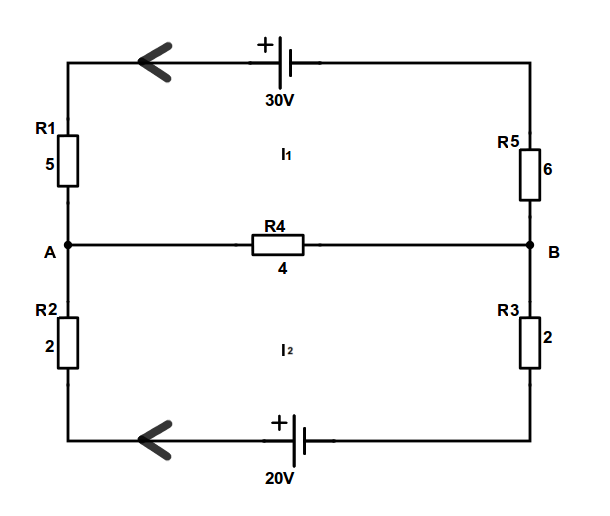
\includegraphics[scale=0.38]{kirchhoff.png}
\end{center}

$I_{1}$ et $I_{2}$ représentent respectivement le courant circulant dans la maille 1 (la pile de 30V, A et B) et le courant circulant dans la maille 2.\\

D’après la loi de Kirchhoff, ou loi des mailles, la somme algébrique des différences de potentiel R.I le long d’une maille orientée est égale à la somme algébrique des tensions aux bornes des générateurs de cette maille orientée.\\

On cherche ici à déterminer les intensités dans les mailles du circuit.

\section{Résolution}

Pour la \textbf{maille 1}, l’intensité $I_{1}$ traverse les résistances R1, R4 et R5. La somme des différences de potentiel R.I est donc de :
\[5I_{1} + 4I_{1} + 6I_{1}= (5+4+6)I_{1} = 15 I_{1}\].
De plus, le courant de la maille 2 traverse aussi la branche A-B de la maille 1. Le sens du courant I2 étant néanmoins opposé au sens du courant I1, on obtient une différence de potentiel de 15 I1 - 4 I2 . La tension dans la maille 1 étant de 30V, on a donc une première équation : 
\begin{equation}
15I_{1}+4I_{2} = 30
\end{equation}        

La méthode est la même pour la \textbf{maille 2}. La différence de potentiel dans la branche AB est donc de 4$I_{1}$ (le sens de $I_{1}$ est le même que celui de $I_{2}$), la somme des résistances de la maille 2 est de $4+2+2=8$.On a donc une deuxième équation :
\begin{equation}
4I_{1}+8I_{2}=20
\end{equation}

On obtient donc le système d'équations linéaires suivant :

\[
\left\{
\begin{array}{r c c l}
15I_{1}+4I_{2} = 30\\
4I_{1}+8I_{2}=20\\
\end{array}
\right.
\]\\


On résout le système à l'aide de la méthode du pivot de Gauss :

\[
\left\{
\begin{array}{r c c l}
4I_{1}+8I_{2}=20\ &  L_1\\
15I_{1}+4I_{2} = 30\ & L_2\\
\end{array}
\right.
\]\\

\[
\left\{
\begin{array}{r c c l}
4I_{1}+8I_{2}=20 & L_1\\
30I_{1}+8I_{2} = 60 & L_2 \leftarrow & 2L_2\\
\end{array}
\right.
\]\\


Ainsi à partir de $L_2$ on obtient $I_{1}$:
$$I_{1}=\frac{40}{26}$$


De même, on remplace $I_{1}$ dans $L_{1}$:
$$I_{2}=\frac{20-4*\frac{40}{26}}{8}$$\\

La méthode du pivot de Gauss nous permet donc d'avoir les valeurs des intensités du circuit:
$$I_{1}=\frac{20}{13}$$
$$I_{2}=\frac{45}{26}$$\\



On observe ainsi que les valeurs de $I_{1}$ et $I_{2}$ sont positives : le courant qui passe dans la maille 1 et celui qui passe dans la maille 2 sont donc dans le même sens que ceux choisis arbitrairement sur le schéma.\\

En utilisant le programme pascal, on peut obtenir les résultats ci-dessous:\\

Système d'équation:\\
\begin{center}
	4.000 $I_{1}$ + 8.000 $I_{2}$ = 20.000\\
	15.000 $I_{1}$ + 4.000 $I_{2}$ = 30.000\\
\end{center}

Système d'équations après la phase d'élimination:\\
\begin{center}
	15.000 $I_{1}$ + 4.000 $I_{2}$ = 30.000\\
	0.000 $I_{1}$ + 6.933 $I_{2}$ = 12.000\\
\end{center}

Solution X:\\
\begin{center}
	$I_{1}$ = 1.538461538461539\\
	$I_{2}$ = 1.730769230769231\\
\end{center}

\newpage
\chapter*{Conclusion}
Pendant ce projet mathématique, nous avons mis en oeuvre des moyens afin de comprendre et d'appliquer la factorisation LU par la méthode de Gauss à un système linéaire. Pour cela, nous avons analyser les différentes possibilités de cette résolution : la méthode de Gauss et l'inverse d'une matrice, vues en M4 et la décomposition sous formes de matrices L et U.\\

La méthode de Gauss est bien adaptée pour la résolution de systèmes d'équations et a l'avantage d'être simple à concevoir et à programmer. Nous avons donc manipuler différents programmes pour appliquer cette résolution à différentes matrices comme la matrice de Hilbert et Wilson. Cependant, nous avons pu remarquer que la machine n'était pas toujours fiable en raison de l'approximation faite pour les nombres à virgule. En effet, nous avons pu prouvé que les deux programmes fournis en début de projet ne sont pas assez précis face à des opérations complexes. L'ordinateur est donc un outil très performant, mais il faut savoir interpréter ses résultats et ne pas s'y fier aveuglément.  \\
\chapter*{Bibliographie}


\textbf{Chapitre 1}\\
Livre \underline{Histoire d'algorithme}, par J.L. Chabert , E. Barbin , M. Guillemot , A. Michel-Pajus. Belin, 2010
\\

\textbf{Chapitre 2}\\
\\
La majeure partie de l’analyse mathématique repose sur l’explication donnée par Mr Gleyse\\

Méthode factorisation A=LU:\\ 
Livre \underline{Méthodes de calcul numérique} - Vol.1 Systèmes d'équations, par Jean-Pierre Nougier. Edition Hermes, 2001\\

\textbf{Chapitre 3}\\
\\
Maltrice de Hilbert : \url{https://fr.wikipedia.org/wiki/Matrice_de_Hilbert}\\
Matrice de Wilson: \url{http://www.math.univ-paris13.fr/~halpern/teaching/MACS1_2010/systemes.pdf}\\
programmes Pascal fournis par Mr. Gleyse\\
Matrice inversible 8*8 : \url{http://palmer.wellesley.edu/~aschultz/summer06/math103/coursenotes_and_handouts/mathematica_060706/}\\


\textbf{Chapitre 4}\\
\\
Utilisation pour les systèmes électriques : programme de P3 (STPI 1)


\end{document}


